\documentclass{article}
\usepackage{tabularx,fullpage,url}
\usepackage[top=1in, bottom=1in, left=.5in, right=.75in]{geometry}
\usepackage{amsmath,amssymb,graphicx,amsthm,xparse, color, mathrsfs} 
\usepackage{ epstopdf, fullpage}

\usepackage[ruled,vlined]{algorithm2e}
\usepackage{xifthen}
\usepackage{wrapfig}

\newcommand{\mypagebreak}{\begin{center}
		\noindent\makebox[\linewidth]{\rule{7.5in}{1pt}}
	\end{center}}
\bibliographystyle{siam}
\newcommand{\minimize}[1]{\underset{#1}{\text{minimize}}}
\newcommand{\maximize}[1]{\underset{#1}{\text{maximize}}}
\newcommand{\mini}[1]{\underset{#1}{\text{min}}}
\newcommand{\argmin}[1]{\underset{#1}{\text{argmin}}}
\newcommand{\st}{\text{subject to}}
\newcommand{\rank}{\textbf{rank}}
\newcommand{\epi}{\mathbf{epi}}

\newcommand{\diag}{\textbf{diag}}
\newcommand{\mb}{\mathbf}
\newcommand{\R}{\mathbb R}
\newcommand{\mle}{\mathbf{MLE}}
\newcommand{\map}{\mathbf{MAP}}
\newcommand{\bE}{\mathbb E}
\newcommand{\mL}{\mathcal L}
\newcommand{\mH}{\mathcal H}
\newcommand{\mB}{\mathcal B}
\newcommand{\mN}{\mathcal N}
\newcommand{\mD}{\mathcal D}
\newcommand{\mC}{\mathcal C}

\newcommand{\mS}{\mathcal S}
\newcommand{\tr}{\mathbf{tr}}
\newcommand{\mrm}{\mathrm}
\newcommand{\proj}{\mathbf{proj}}
\newcommand{\prox}{\mathbf{prox}}
\newcommand{\sign}{\mathbf{sign}}
\newcommand{\range}{\mathbf{range}}
\newcommand{\var}{\mathbf{var}}
\newcommand{\vnull}{\mathbf{null}}
\newcommand{\pr}{\mathbf{Pr}}
\newcommand{\find}{\mathbf{find}}
\newcommand{\argmax}[1]{\underset{#1}{\mathrm{argmax}}}
\newcommand{\subjto}{\mathrm{subject~to}}


\newcommand{\red}[1]{{\color{red}#1}}
\newcommand{\blue}[1]{{\color{blue}#1}}

\newcommand{\gray}[1]{\textcolor{lightgray}{#1}}



\newcommand{\idx}[1]{{\scriptsize [#1]}}

\newcommand{\showpoints}[1]{\textbf{(#1)}}


\begin{document}
{\Large\textbf{CSE 353: Homework 4 \hfill
Due Friday  Nov. 4}}


\mypagebreak

\begin{enumerate}



\item \emph{Machine learning fundamentals.}  \showpoints{3 pts, 1 pt each}


\begin{tabular}[t]{lll}
\begin{minipage}{.7\linewidth}
There is a growing need for machine models to have \emph{interpretability}; that is, when it tells you the label of your new data sample, you want to also understand \emph{why} it told you this. One of the most common answers to the ``why" is to find which features (or which combination of features) best contributed to the answer given, or which samples best contributed to the model. In each case, describe how you could use parts of the learned model to return not only a new data label, but which features (or samples) were most important. Be specific and detailed; if I can't implement your suggestion based on what you wrote, you won't get full credit. 

\begin{enumerate}
\item  Decision trees


\item Linear regression



\item Support vector machines.


\end{enumerate}
\end{minipage}
&$\;$&
\begin{minipage}{.3\linewidth}
\centering

\includegraphics[width=\linewidth]{figs/machine_learning.png}\\(source: xkcd)
\end{minipage}
\end{tabular}




\item \emph{Adaboost}\showpoints{3pts}
A popular and computationally cheap boosting method is adaboost, described in Algorithm \ref{alg-adaboost}. In particular, it is a greedy coordinate-wise method that minimizes the empirical exponential loss, e.g. given a predictor $h(x) = y$, we find $h$ which minimizes
\[
f(h) = \frac{1}{m}\sum_{i=1}^m \exp(-y_ih(x_i)).
\]
 In this problem, we will implement Adaboost and analyze its greedy structure.



\begin{algorithm}[H]
\SetAlgoLined
\KwData{Samples: $x_1,...,x_m$, training labels $y_i\in \{-1,1\}$, weak learners $\mH$.}
\KwResult{Classifier $H(x) = \sum_{t=1}^T \alpha_t h^{(t)}(x)$}
 Initial weights $w_i^{(0)} = \frac{1}{m}$ for $i = 1,...,m$\;
 \For{$t=1,...,T$}{
 
	Choose $h^{(t)}(x)$ which minimizes the weighted sum error for misclassified points 
	\[
	h^{(t)}(x) = \argmin{h\in \mH}\; \sum_{\substack{i=1\\ h(x_i)\neq y_i}}^m  w_i^{(t-1)}
	\]\\
	Update 
	\[
	\alpha^{(t)} = \frac{1}{2} \log\left(\frac{1-\epsilon^{(t)}}{\epsilon^{(t)}}\right), \qquad \epsilon^{(t)} :=\sum_{h^{(t)}(x_i)\neq y_i} w^{(t-1)}_i \qquad (\star)
	\]
	\\
	
	
	Update weights 
	\[
	\hat w_i^{(t)} = w_i^{(t-1)}\exp(-y_i\alpha^{(t)} h^{(t)}(x_i)), \qquad w_i^{(t+1)} = \frac{\hat w_i^{(t+1)}}{\sum_j \hat w_j^{(t+1)}}
	\]

 }
 \caption{Discrete Adaboost (source: https://en.wikipedia.org/wiki/AdaBoost)
}
\label{alg-adaboost}
\end{algorithm}







\begin{enumerate}




\item Open the mnist\_adaboost\_release directory and in the iPython notebook, download the data. We are again going to do 4/9 handwriting disambiguation. Only minimal preprocessing was used in this dataset. You may now use sklearn's tree implementation.

\begin{itemize}
\item Write a function that computes the train and misclassification rates , as well as the train exponential loss value, using just this decision stump (tree of depth = 1). 
Over the given dataset, these values should be:
\[
10.98\% \text{ train misclassification}, 
15.27\% \text{ test misclasification},
0.6259675480492947 \text{ exponential loss}
\]


\item \textbf{Deep trees.} Using the tree library from sklearn, train trees with depth 1 to 100, and plot the train and test misclassification rate, as well as the train exponential loss, as a function of depth. Report also the smallest  train and test misclassification rate, and smallest train exponential loss, over the sweep.


\item \textbf{Boosted decision stumps.} \showpoints{1 pt} Now build  a decision stump, e.g. a tree with depth = 1. Initialize weights as $w_i = 1/m$ for all $i = 1,...,m$, and fit the decision tree over the \emph{weighted} misclassification error, using the code snippet

\begin{center}
\texttt{clf = clf.fit(Xtrain, ytrain, sample\_weight = w)}.
\end{center}




\item  \showpoints{1 pt}
Implement the Adaboost method, as shown in algorithm \ref{alg-adaboost}. Plot the training exponential loss, and train and test misclassification  rate. 
Report also the smallest  train and test misclassification rate, and smallest train exponential loss, over the sweep. Comment on how the boosted decision stumps performed compared to the deep decision tree.




\item \showpoints{1 pt}
Plot also $\epsilon^{(t)}$ and $\alpha^{(t)}$ as a function of $t$. For what values of $\epsilon^{(t)}$ is $\alpha^{(t)}$ really large and positive? really large and negative? close to 0? Interpret this mechanism; what is it saying about how boosting uses classifiers, in terms of their weighted performance?





\end{itemize}



\end{enumerate}


\item \emph{Polyfit via linear regression.} \showpoints{4 pts } 

\begin{itemize}
\item Download weatherDewTmp.mat. Plot the data. It should look like the following
\begin{center}
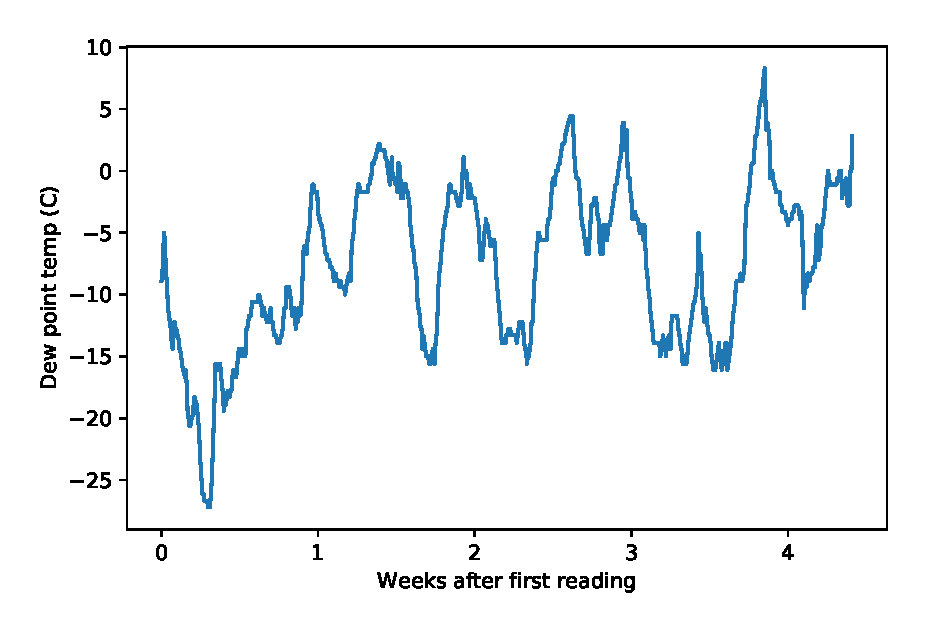
\includegraphics[width=3in]{polyfit_figs/polyfit_hw1_0.eps}
\end{center}


\item We want to form a polynomial regression of this data. That is, given $w = $ weeks and $d$ = dew readings, we want to find $\theta_1,...,\theta_p$ as the solution to
\begin{equation}
\underset{\theta\in \mathbb R^p}{\text{minimize}} \quad \tfrac{1}{2}\sum_{i=1}^m (\theta_1 + \theta_2 w_i + \theta_3 w_i^2 + \cdots + \theta_{p} w_i^{p-1} - d_i)^2.
\label{eq:polyfit0}
\end{equation}
Form $X$ and $y$ such that \eqref{eq:polyfit0} is equivalent to the least squares problem
\begin{equation}
\underset{\theta\in \mathbb R^p}{\text{minimize}} \quad \tfrac{1}{2}\|X\theta - y\|_2^2.
\label{eq:polyfit1}
\end{equation}
That is, for $w$ the vector containing the week number, and $y$ containing the dew data, form 
\[
X = \begin{bmatrix}
1 & w_1 & w_1^2&  w_1^3 &\cdots &w_1^{p-1}\\
\vdots& \vdots & \vdots & \ddots & \vdots\\
1 & w_m & w_m^2&  w_m^3 &\cdots &w_m^{p-1}\\
\end{bmatrix}.
\]

\end{itemize}
\begin{enumerate}
\item  \emph{Linear regression.}\showpoints{1pt} 
\begin{enumerate}
\item Write down the normal equations for problem \eqref{eq:polyfit1}. 

\item Fill in the code to solve the normal equations for $\theta$, and use it to build a predictor.
To verify your code is running correctly, the number after \texttt{check number} should be   $1.759$ (implemented correctly) or $1.341$ (also accepted).


\item Implement a polynomial fit of orders $p = 1,2,3,10,100$, for the weather data provided. Include a figure that plots the original signal, overlaid with each polynomial fit. Comment on the ``goodness of fit" for each value of $p$.


\end{enumerate}
\item \emph{Ridge regression.}\showpoints{1pt}   Oftentimes, it is helpful to add a \emph{regularization term} to \eqref{eq:polyfit1}, to improve stability.  In other words, we solve 
\begin{equation}
\underset{\theta\in \mathbb R^p} {\text{minimize}}\quad \tfrac{1}{2}\|X\theta - y\|_2^2 + \tfrac{\rho}{2} \|\theta\|_2^2.
\label{eq:polyfit2}
\end{equation}
for some $\rho > 0$. 
\begin{enumerate}
\item Again, write down the normal equations for \eqref{eq:polyfit2}. Your equation should be of form $A\theta =b$ for some matrix $A$ and vector $b$ that you specify.





\item Write the code for solving the ridge regression problem and run it. To verify your code is running correctly, the number after \texttt{check number} should be   $1.206$.

\item  Using $\rho = 1.0$,  plot the weather data with overlaying polynomial fits with ridge regression. Provide these plots for $p = 1,2,3,10,100$. Comment on the ``goodness of fit" and the stability of the fit, and also compare with the plots generated without using the extra penalty term. 


\end{enumerate}

\item \emph{Conditioning.} \showpoints{1pt} 
\begin{enumerate}
\item An \emph{unconstrained quadratic problem} is any problem that can be written as
\begin{equation}
\minimize{\theta}\quad \frac{1}{2}\theta^TQ\theta + c^T\theta + r
\label{eq:quadratic_problem}
\end{equation}
for some symmetric positive semidefinite matrix $Q$, and some vector $c$ and some scalar $r$. Show that the ridge regression problem \eqref{eq:polyfit2} is an unconstrained quadratic problem by writing down $Q$, $c$, and $r$ in terms of $X$ and $y$ such that
\eqref{eq:quadratic_problem} is equivalent to \eqref{eq:polyfit2}.


\item In your code, write a function that takes in $X$ and $y$, constructs $Q$ as specified in the previous problem, and  returns the condition number of $Q$. Report the condition number $\kappa(Q)$ for varying values of $p$ and $\rho$, by filling in the following table. 
Here, $m = 742$ is the total number of data samples. Report at least 2 significant digits.
Comment on how much ridge regression is needed to affect conditioning.

\begin{center}
\begin{tabular}{|l||l|l|l|l|}\hline
p& $\rho = 0$   & $\rho = m$   &$\rho = 10m$   &$\rho = 100m$\\ 
\hline\hline
1&  &&&\\
\hline
2&  &&&\\\hline
5&  &&&\\\hline
10& &&&\\\hline
\end{tabular}
\end{center}






\item Under the \emph{same experimental parameters} as the previous question, run ridge regression for each choice of $p$ and $\rho$, and fill in the table with the mean squared error of the fit:
\[
\textbf{mean squared error} = \frac{1}{m}\sum_{i=1}^m (x_i^T\theta - y\idx{i})^2
\]
where $x_i$ is the $i$th row of $X$.
Comment on the tradeoff between using larger $\rho$ to improve conditioning vs its affect on the final performance. 


\begin{center}
\begin{tabular}{|l||l|l|l|l|}\hline
p& $\rho = 0$   & $\rho = m$   &$\rho = 10m$   &$\rho = 100m$\\ 
\hline\hline
1&  &&&\\
\hline
2&  &&&\\\hline
5&  &&&\\\hline
10& &&&\\\hline
\end{tabular}
\end{center}





\end{enumerate}
\item \emph{Forcasting.} \showpoints{1pt}  Picking your favorite set of hyperparameters ($p$, $\rho$), forecast the next week's dew point temperature. Plot the forecasted data over the current observations. Do you believe your forecast? Why?







\end{enumerate}











\end{enumerate}




\end{document}